\section{Representation Types}
\label{sec:representation_types}

This chapter gives an overview of different ways for representing a tour of a TSP instance. We furthermore define which representation types will be used in our experiments.
There are different possible representations for a tour of a TSP instance, namely:

\begin{itemize}
	\item Binary representation
	\item Matrix representation
	\item Path representation (Section \ref{subsec:path})
	\item Ordinal representation (Section \ref{subsec:ordinal})
	\item Random-key representation (Section \ref{subsec:random_key})
	\item Adjacency representation (Section \ref{subsec:adjacency})
\end{itemize}

According to \citeauthor{larranaga1999genetic} \cite{larranaga1999genetic}, the first two options are a standard way of representation used in genetic algorithms. However, in case of the TSP, applying crossover and mutation operators on them does not guarantee to result in valid tours. Therefore, they have been excluded from our subsequent considerations.

\subsection{Path Representation}
\label{subsec:path}

The path  representation  is  the  most  natural  representation  of  a  tour.  For  example, a tour $\pi = (0, 1, 2, 3, 4)$ is represented by the path $0\rightarrow1\rightarrow2\rightarrow3\rightarrow4\rightarrow0$. From now on, we will use the shorthand notation 01234 for examples with less than ten nodes for this representation type, where it is implicitly assumed that there exists an edge from the last city to the first one.
This representation leads to several chromosomes which represent the same tour because the start city can be different. Therefore, all these chromosomes have the same fitness value and can thus be considered as equivalent.\par

Note that this representation for a TSP tour can provoke problems when applying classical operators of genetic algorithms. For instance, the classical one-point crossover takes one cut point and defines the offspring by taking the part before the cut point from the first parent and the part after the cut point from the second parent. When using the path representation, the result is not necessary a valid tour.  For instance, a one-point crossover for the chromosomes 051243 and 541203 may result in the offspring 051203 (see Figure \ref{one_point_crossover}).  However, city 0 appears twice in the offspring while city 4 does not appear at all. It is obvious that the offspring does not represent a valid tour. This representation therefore requires additional measures to avoid such duplicates. Nevertheless, the simplicity of this representation has caused its large applicability. Moreover, there is a large number of operators for the path representation which ensure the validity of the offspring (see Section \ref{subsec:path_crossovers}). For this reason, we will use the path representation in our experiments.

\begin{figure}[htp] \centering
	\centering
	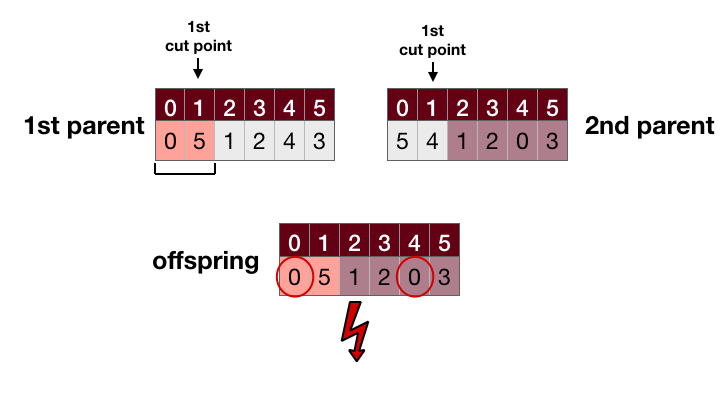
\includegraphics[width=0.6\textwidth]{one_point_crossover}
	\caption{One-point crossover for chromosomes 051243 and 541203 in the path representation.}
	\label{one_point_crossover}
\end{figure}

\subsection{Ordinal Representation}
\label{subsec:ordinal}

The ordinal representation was proposed by \citeauthor{grefenstette1985genetic} \cite{grefenstette1985genetic}. A tour in the ordinal representation is given as a list of $n$ cities. Moreover, there exists a so-called "reference tour" which represents an ordered list of cities to decode and encode the tour in this representation. In order to get an ordinal representation, one has to go through the given tour and identify the position which the next city occupies in the reference tour. This index is used as the next element in the ordinal representation. After that, this city is deleted from the reference tour. An analogous procedure can be used to decode the ordinal representation.\par

\begin{figure}[htp] \centering
	\centering
	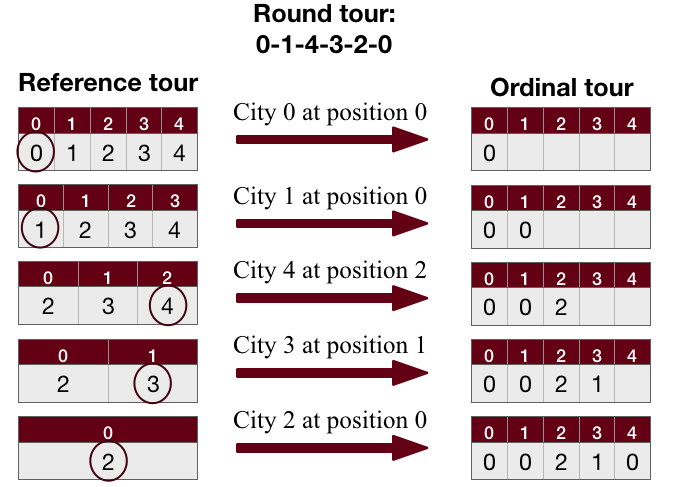
\includegraphics[width=0.6\textwidth]{repr_ordinal}
	\caption{Ordinal representation for a tour $\pi = (0, 1, 4, 3, 2)$.}
	\label{repr_ordinal}
\end{figure}


For instance, let us consider the tour $\pi = (0, 1, 4, 3, 2)$ (see Figure \ref{repr_ordinal}). We use the ascendingly ordered list of cities as reference tour $ref=(0, 1, 2, 3, 4)$. To get an ordinal representation, we have to go through the cities of $\pi$ and define their positions in $ref$. The first city of the tour is the city $0$ which occupies the 0th position in the reference tour. We delete this city from the reference tour, getting $ref=(1, 2, 3, 4)$ and $ordinal = (0)$. The next city of tour $\pi$ is city 1 which stands now at the position 0 in the reference tour; therefore, 0 is added to the ordinal representation. After deleting city 1 from the reference tour, we get $ref=(2, 3, 4)$ and $ordinal = (0, 0)$. City 4 is the next one and it takes position 2 in the reference tour. Thus, we get $ref=(2, 3)$ and $ordinal = (0, 0, 2)$. City 3 has position 1, resulting in $ref=(2)$ and $ordinal = (0, 0, 2, 1)$. The last city in $\pi$ is city 2 which stands at the position 0 of the reference tour. Therefore, 0 is added to the ordinal representation, and we finally get $ref=()$ and $ordinal = (0, 0, 2, 1, 0)$. \par 

We will now show how the decoding procedure works. Having the ordinal tour  $ordinal = (0, 0, 2, 1, 0)$ and the reference tour $ref=(0, 1, 2, 3, 4)$, the first number in the ordinal representation is 0. This means that if we want to get the first city of the original tour, we need to get the element in the reference tour which stands at the position 0 and remove it from the reference tour after that. So, we get the city 0, obtaining the partial tour $\pi = (0)$ and $ref=(1, 2, 3, 4)$. The next element in the ordinal representation is 0 as well. This means that we have to look for a city again at the position 0 in the reference tour. Now it is city 1. As a result, we get the partial tour $\pi = (0, 1)$ and $ref=(2, 3, 4)$. The next element of the ordinal tour, namely 2, brings us to the city 4 which stands at this position in the reference tour, resulting in the partial tour $\pi = (0, 1, 4)$ and $ref=(2, 3)$. After that, we find the city 3 at the position 1, leaving us with $\pi = (0, 1, 4, 3)$ and $ref=(2)$. The last element of the ordinal tour is 0.  This will always be the case because the reference tour only consists of a single element now. City 2 is this remaining city in the reference tour, and it finishes the round tour $\pi$. Thus, the original tour is $\pi = (0, 1, 4, 3, 2)$.\\

\citeauthor{potvin1996genetic} \cite{potvin1996genetic}  showed that if a classical one-point crossover (which did not work for the path representation) is applied in this representation, the generated offspring will always represent a valid tour. He explained it by the fact that each value in the ordinal tour corresponds to a particular position in the reference tour. While applying a one-point crossover, exchanging values between two parent chromosomes simply modifies the order of selection of the cities in the reference tour. Therefore, a valid permutation is always generated. \citeauthor{larranaga1999genetic} \cite{larranaga1999genetic} pointed out that the partial tours to the left of the cut point do not change, whereas the partial tours to the right of it are disrupted in a quite a random way. According to \citeauthor{larranaga1999genetic} \cite{larranaga1999genetic}, these disruptions are the reason for relative poor results which this representation type has shown. Also \citeauthor{potvin1996genetic} \cite{potvin1996genetic} has also pointed out that this representation type can be considered mainly out of historical interest because the sequences of cities in the parents are not well inherited in the offspring, resulting in mostly random permutations. We are going to consider this representation type in our experiments to find out whether it shows bad performance on our data set as well. \par 

\subsection{Random-Key Representation}
\label{subsec:random_key}

The concept of \textit{random keys} for representing round tours was proposed by \citeauthor{bean1994genetic} \cite{bean1994genetic}. This representation uses random numbers typically drawn uniformly from the interval $[0, 1)$. Each chromosome consists of a list of such randomly drawn numbers. It is assumed that the $i$th random number is associated with city $i$. By sorting the chromosomes in ascending \cite{bean1994genetic} or descending \cite{knust2020script} order, one can thus obtain a valid permutation of the cities. \par

For instance, let us assume that we have drawn the following random keys which encode a tour of length 5 : $keys=(0.47, 0.05, 0.34, 0.99, 0.55)$. Now, we assign these random numbers to the cities, namely: $0.47 \rightarrow 0, 0.05 \rightarrow 1, 0.34 \rightarrow 2, 0.99 \rightarrow 3, 0.55 \rightarrow 4$. Then, we sort the keys in ascending order and get:
$sorted$ =(0.05(1), 0.34(2), 0.47(0), 0.55(4), 0.99(3)). Therefore, the decoded tour is $\pi = (1, 2, 0, 4, 3)$.\par 

According to \citeauthor{snyder2006random} \cite{snyder2006random}, the random-key representation is useful for problems that require permutations of integers where traditional crossovers have problems with producing valid offsprings (as, for instance, a one-point crossover in the path representation, as described above in Section \ref{subsec:path}). Standard crossover techniques applied in this representation will generate children that are guaranteed to be valid.\par 

Nevertheless, in our implementation, we do not work with the random-key representation because we use construction heuristics to produce chromosomes for the initial population. These heuristics return round tours in the path representation. There is, however, an infinite number of ways to translate a tour from the path representation into the random-key representation: We need to ensure that the keys are ordered in the correct way, but the numerical value of the keys is not determined. The actual numeric value does, however, play a critical role when applying crossover and mutation operators in this representation. As it is unclear how to translate the initial population from the path representation to the random-key representation, we do not consider the latter in our experiments.\par 


\subsection{Adjacency Representation}
\label{subsec:adjacency}

In this representation type, each array index represents one city. If the value $j$ is found at index $i$ of the array, this means that the round tour contains an edge $(i, j)$ from city $i$ to city $j$.  In the path representation, we have a designated starting point which results in $n$ chromosomes representing the same round tour. In contrast to that, there is no designated starting point in the adjacency representation, but this representation type is directed. For symmetric TSP instances, the same round tour which goes in one direction will look different from the one which goes in the opposite direction. Therefore, each round tour can be mapped to two chromosomes for symmetric TSP instances and exactly to one chromosome for asymmetric TSP instances in adjacency representation.
\begin{figure}[htp] \centering
	\centering
	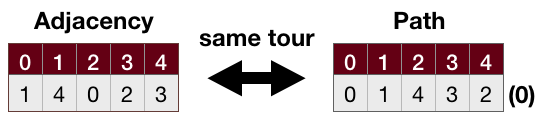
\includegraphics[width=0.5\textwidth]{Adj_Path}
	\caption{The same round tour in path and adjacency representation. }
	\label{Adj_Path}
\end{figure}

One can easily transform a tour in this representation into the path representation (see Figure \ref{Adj_Path}): City 0 is always added to the path tour at the beginning automatically. Then, one starts at the index 0 and looks which city stands at this index in the adjacency representation. This city becomes the next city of the path tour. After that, this city is used as the next index and the city which takes this index continues the path tour. The process repeats until the whole path is build. For instance, consider the tour 14023 in the adjacency representation. In the adjacency representation, we find city 1 at the index 0 which means that city 0 is followed by city 1 in the round tour. We thus append it to our path. At the index 1, stands city 4, which is added to the path. At the index 4, we find city 3. Its neighbor is city 2, as it stands at the index 3. City 0 is at the index 2 which completes the Hamilton cycle 01432(0) in the path representation.\par 

 An inverse transformation from the path representation into the adjacency representation is possible as well. One goes along the path tour and for each pair of neighbors $\pi_{i}$ and $\pi_{i + 1}$ in the path tour $\pi = (\pi_{1},...,\pi_{i},\pi_{i + 1},...\pi_{n})$, city $\pi_{i + 1}$ takes index $\pi_{i}$ in the adjacency representation. For instance, let us reuse the example in Figure \ref{Adj_Path}. We have the tour 01432 in the path representation. The first pair of cities includes 0 and 1. This means that city 1 takes position 0. The next pair contains cities 1 and 4, resulting in that city 4 takes position 1 in the adjacency representation. In the same way, city 3 takes position 4, and city 2 takes position 3. As a round tour is needed in case of TSP instances, we need to make a connection between city 2 and 0. Therefore, city 0 stands at the position 2 and finishes the tour.\par 

Please note that like the path representation also the adjacency representation needs special operators to preserve the validity of the chromosomes (see Section \ref{subsec:adjacency_crossovers}). We included this representation type with its specific crossover operators in our implementation to compare its effectiveness with the one of the path representation. As a translation from the path representation to the adjacency representation is quite straightforward, we can also use the tours found by the construction heuristics with this representation type.\par 